\documentclass{article}
\usepackage[UTF8]{ctex}
\usepackage{float} %设置图片浮动位置的宏包
\usepackage{graphicx} %插入图片的宏包
\usepackage{subfigure} %插入多图时用子图显示的宏包
\usepackage{newtxtext}
\usepackage{indentfirst}
% 加载tikz宏包
\usepackage{tikz}
\usepackage{geometry}

\geometry{
	a4paper,
	total={170mm,257mm},
	left=20mm,
	top=20mm,
}

\begin{document}
\begin{center}
	{\CJKfamily{hei} \CJKfamily{Times New Roman} \fontsize{16pt}{20pt}\selectfont \textbf{去年今日此门中,人面桃花相映红。\\人面不知何处去,桃花依旧笑春风。}}
\end{center}
\begin{figure}[H]
	\centering
	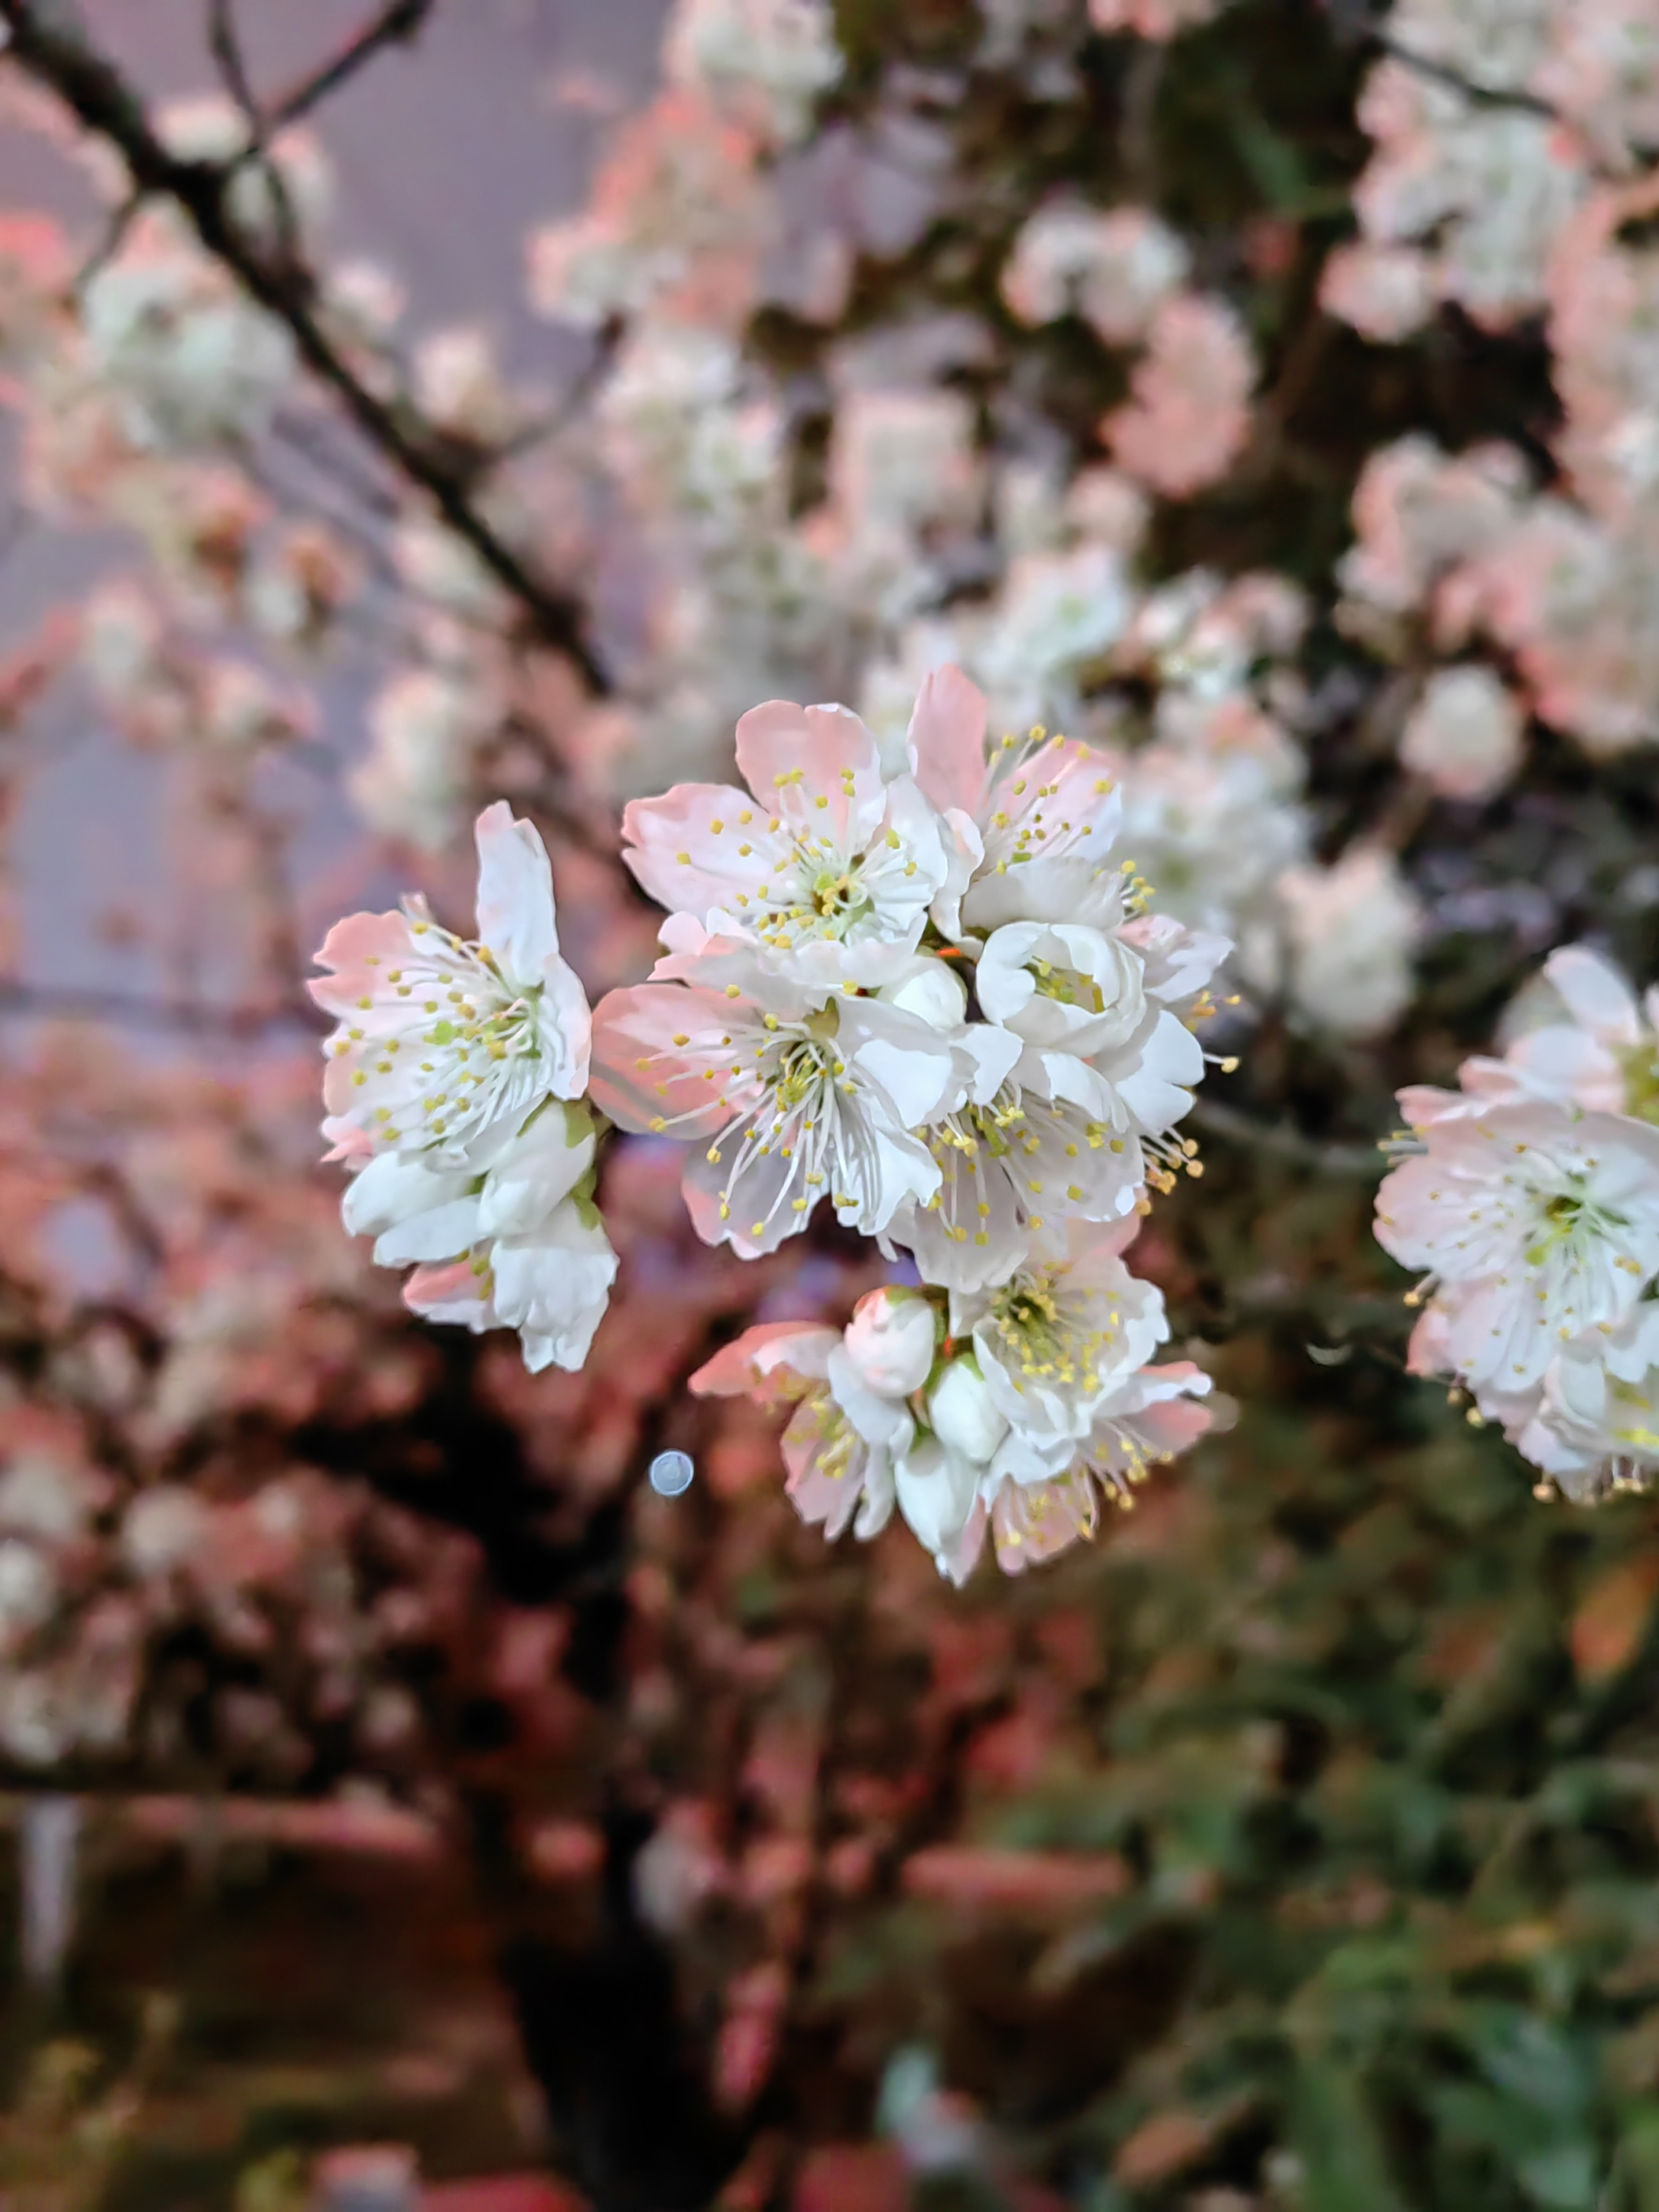
\includegraphics[width=15cm]{./img/index.png}% 图片相对位置
	\caption{\CJKfamily{hei} \CJKfamily{Times New Roman} 2023年3月10日.你见到我了吗?} % 图片标题 
\end{figure}

\newpage
\emph{\large “你以为这天又是一个很平常的日子,多年之后才发现,这其实是你人生里最棒的一天。这样的一天永远不会再有了。” }

\vspace{1.5pt}
\noindent\hrulefill
\begin{flushright}
	\textit{xingchenziyi@163.com}
	\\\textit{\textbf{李星辰同学}}
\end{flushright}

%\noindent 你还会记得我吗?
\newpage
\begin{center}
	{\CJKfamily{hei} \CJKfamily{Times New Roman} \fontsize{16pt}{20pt}\selectfont 基于双目视觉的室内移动机器人SLAM技术研究}
\end{center}
\tableofcontents
\section{引言}

\subsection{项目简介}
\subsection{软件结构}
\subsection{硬件结构}
\subsection{机械结构}
\subsection{项目流程}

\section{实验建模}
\subsection{软件设计}
\subsection{硬件设计}
\subsection{机械设计}
\subsubsection{室内移动机器人建模}
\subsection{仿真模拟}

\section{实验结果的分析与检验}
\subsection{实验结果}
\subsection{模型检验}
\subsection{实验总结}

\section{未来和展望}
\subsection{应用场景}
\subsection{实验改进}

\section{参考文献}
\end{document} 

